% !TeX spellcheck = es_ES
\documentclass[12pt, titlepage]{article}
\usepackage[nottoc,notlot,notlof,numbib]{tocbibind}
\usepackage[letterpaper, margin=2.5cm]{geometry}
\usepackage[utf8]{inputenc}
\usepackage[spanish]{babel}
\usepackage{listings}
% imagenes
\usepackage{graphicx} 
\usepackage{float}
% fin imagenes
\usepackage{url}
\usepackage{color}
\usepackage{amsmath}
\usepackage{bm}

\definecolor{dkgreen}{rgb}{0,0.6,0}
\definecolor{gray}{rgb}{0.5,0.5,0.5}
\definecolor{mauve}{RGB}{253,151,31}
\definecolor{deepred}{RGB}{249,38,114}

\lstset{frame=tb,
	language=MATLAB,
	aboveskip=3mm,
	belowskip=3mm,
	showstringspaces=false,
	columns=flexible,
	numbers=left,
	stepnumber=1,
	basicstyle={\small\ttfamily},
	numberstyle=\tiny\color{gray},
	keywordstyle=\color{blue},
	commentstyle=\color{dkgreen},
	stringstyle=\color{mauve},
	breaklines=true,
	breakatwhitespace=true,
	tabsize=2,
	morekeywords={self, append},
	emph={},
	emphstyle=\color{deepred}
}

\title{Reporte de la red de Hamming}
\author{Barrera Pérez Carlos Tonatihu \\ Boleta: 2016630023 \\ Profesor: Moreno Armendariz Marco Antonio \\ Redes Neuronales \\ Grupo: 3CM2 }
\begin{document}
    \maketitle
    \tableofcontents
    \newpage
    \section{Introducción}
    Esta práctica es sobre una red competitiva, la red de Hamming, el contenido de este reporte incluye una introducción a la teoría detrás del funcionamiento y estructura de dicha red donde el principal componente  tratar es su arquitectura y su modelo matemático lo cual es indispensable para entender los ejemplos planteados en la parte de resultados de experimentos.
    
    En esta parte se presentan las pruebas que se realizaron para verificar el funcionamiento de dicha red y poder observar su comportamiento con el objetivo de poder apreciar la aplicación que se le puede dar a dicha red.
    
    Para continuar con este análisis de resultados se presenta una sección de discusión de resultados con observaciones importantes que surgieron del estudio de los valores y gráficas obtenidos en la sección anterior.
    
    Al terminar este análisis es importante mencionar en que casos se podría aplicar y las diferentes ventajas o desventajas que presenta y el porque de su estudio es importante, esto se trata en la sección de conclusiones.
    
    El resto del reporte incluye la bibliografía consultada para el desarrollo de la práctica y el código que fue usado en la misma el cual fue elaborado usando el lenguaje MATLAB.
    \newpage
    \section{Marco teórico}
    La red Hamming es una arquitectura capaz de reconocer patrones binarios. Está formada por dos capas como se muestra en la figura \ref{fig:hamming-diagrama}. La primera capa es una capa de propagación hacia adelante (feedforward en ingles), esto quiere decir que los datos de entrada solamente pueden avanzar de su entrada a la salida de la red nunca en sentido opuesto. \cite{hammi}
    La expresión correspondiente a esta capa es la siguiente.
    \[ a^1=purelin(W^1p+b^1) \]
    donde $a^1$ es la salida de la capa, $W^1$ es la matriz de pesos, $p$ es el vector de entrada y $b^1$ es el bias.
    \begin{figure}[H]
        \begin{center}
            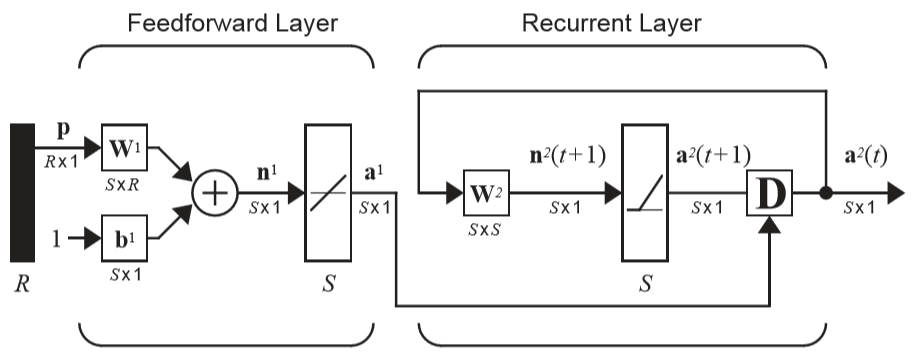
\includegraphics[width=16cm]{img/hamming/diagrama.png}
            \caption{Estructura de la red de Hamming. \cite{libro1}}
            \label{fig:hamming-diagrama}
        \end{center}
    \end{figure}
    En la siguiente capa, la capa recurrente, es donde se realiza una competición con la cual se puede determinar que vector prototipo es el más parecido al vector de entrada.\cite{libro1}
    Es por esto que esta red es de tipo competitiva además de que es de las redes más simples en su categoría.
    Esta capa tiene como expresión matemática a:
    \[\boldsymbol{a^2(t+1) = poslin(W^2a^2(t))}\]
    En esta capa se produce una inhibición lateral, esto quiere decir que la salida de cada neurona tiene un efecto inhibitorio sobre el resto de las neuronas lo cual se ve reflejado en el funcionamiento de la red donde a medida que avanza el valor de alguna neuronas disminuye más lento que el resto. \cite{libro1} 
    
    La construcción de una red de Hamming que reconozca un grupo de vectores prototipo es la siguiente:
    \begin{enumerate}
        \item Si tenemos un conjunto de vectores prototipo como el siguiente.
        \[ \left\lbrace \boldsymbol{p_1, p_2, ..., p_Q} \right\rbrace  \]
        La transpuesta de estos vectores sirven para llenar la matriz de pesos de la primera capa $W^1$ de la siguiente forma.
        \[\boldsymbol{ W^{1}} = \left[\begin{array}{c}\boldsymbol{p^{T}_1}\\\boldsymbol{ p^{T}_2}\\ \vdots \\ \boldsymbol{p^{T}_Q}\end{array}\right]  \]
        \item Por otro lado el bias es llenado con el tamaño $R$ de los vectores prototipo, es decir,
        \[ \boldsymbol{b^{1}} = \left[\begin{array}{c}R\\ R\\ \vdots \\ R\end{array}\right] \]
        \item Para la siguiente capa debido a que es una capa recurrente debemos de inicializar la capa recurrente con el valor de salida de la capa feedforward, es decir, $\boldsymbol{a^2(0) = a^1}$, esto con el fin de poder obtener los siguientes valores de la forma 
        \[  \boldsymbol{a^2(t+1) = poslin(W^2a^2(t))}\]
        \item Lo siguiente es llenar la matriz de pesos de la segunda capa en donde los elementos en la diagonal de la matriz tendrán valores de uno y el resto serán valores pequeños negativos.
        \[ f(i, j) = 
        \begin{cases} 
        minimo(f(i, j-1), f(i+1, j)) & i < j \mathbin{\&}  P_{i} \ne  P_{j} \\
        f(i+1, j-1) + 1 & i < j  \mathbin{\&}  A_{i} =  B_{j} \\
        0 & \text{en otro caso}
        \end{cases} \]
        El valor de épsilon se obtiene por la siguiente formula: $ 0 < \epsilon <\frac{1}{S-1}$ donde $S$ es el número de neuronas
        \item Finalmente, solo se tiene que introducir un vector en la entrada de la primera capa, propagar hacia adelante y utilizar la recurrencia de la segunda capa hasta que solo una salida de esta capa tenga un valor positivo, el indice de la salida indica que vector prototipo reproduce dicha salida.
    \end{enumerate}
\newpage
    \section{Resultados experimentales}
    \textbf{Experimento 1}. Es importante señalar que la asignación de valores se realizo a través de un archivo de texto llamado \emph{entrada\_hamming.txt}
    \begin{figure}[H]
        \begin{center}
            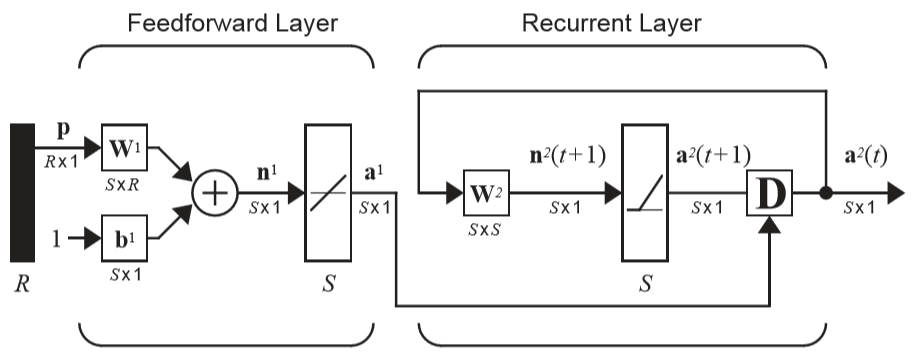
\includegraphics[width=16cm]{img/hamming/diagrama.png}
            \caption{Estructura de la red de Hamming. \cite{libro1}}
            \label{fig:hamming-diagrama2}
        \end{center}
    \end{figure}
    Para hacer la primera prueba sobre la red Hamming se utilizo el siguiente conjunto de vectores prototipo.
    \[ \left\lbrace \boldsymbol{p_1} = \left[\begin{array}{c}-1\\ 1\\ -1\end{array}\right], \boldsymbol{p_2} = \left[\begin{array}{c}-1\\ -1\\ 1\end{array}\right], \boldsymbol{p_3} = \left[\begin{array}{c}1\\ 1\\ -1\end{array}\right], \boldsymbol{p_4} = \left[\begin{array}{c}1\\ -1\\ -1\end{array}\right] \right\rbrace \]
    Y el vector de a clasificar fue el siguiente.
    \[ \boldsymbol{p} = \left[\begin{array}{c}-1\\ 1\\ -1\end{array}\right] \]
    Por lo que la arquitectura definida en la figura \ref{fig:hamming-diagrama2} tiene los siguientes valores.
    \begin{align*}
    R = 3 \implies \boldsymbol{b} = \left[\begin{array}{c}3\\ 3\\ 3\end{array}\right] && S = 4 && \boldsymbol{W} = \left[\begin{array}{c}\boldsymbol{p^{T}_1}\\ \boldsymbol{p^{T}_2}\\ \boldsymbol{p^{T}_3} \\ \boldsymbol{p^{T}_4}\end{array}\right]
    \end{align*}
    Al aplicar estos valores a nuestra red la capa recurrente termino en la iteración 13 y convergió exitosamente a la clase 1 que es la que se esperaba que convergiera.
    %modelo matemático, arquitectura, conjunto de entrenamiento, condición de finalización, valores finales de w y bias
    \begin{figure}[H]
        \begin{center}
            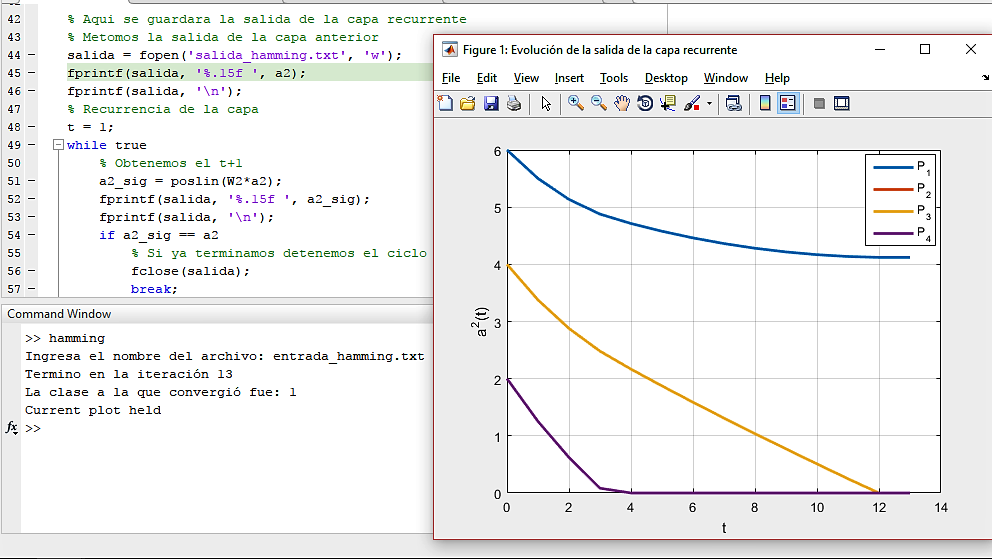
\includegraphics[width=16cm]{img/hamming/hamming1.png}
            \caption{Prueba 1 de la red Hamming.}
            \label{fig:hamming1}
        \end{center}
    \end{figure}
    En la figura \ref{fig:hamming1} se puede observar que solo la curva asociada a la neurona 1 de la capa recurrente que corresponde al vector prototipo 1 es la única que tiene un valor distinto de 0.
    \newline
    \textbf{Experimento 2.}
    En esta segunda prueba se utilizo el siguiente conjunto de vectores prototipo.
    \[ \left\lbrace \boldsymbol{p_1} = \left[\begin{array}{c}1\\ -1\\ -1 \\ -1 \end{array}\right], \boldsymbol{p_2} = \left[\begin{array}{c}-1\\ -1\\ -1 \\ 1 \end{array}\right] \right\rbrace \]
    El vector de prueba a clasificar fue el siguiente.
    \[ \boldsymbol{p} = \left[\begin{array}{c}1\\ 1\\ -1 \\ -1\end{array}\right] \]
    Los valores fueron ingresados mediante un archivo de texto llamado \emph{entrada\_hamming2.txt}. Esto dio como resultado que los valores de la red Hamming de la figura \ref{fig:hamming-diagrama2} sean los siguientes.
    \begin{align*}
    R = 4 \implies \boldsymbol{b} = \left[\begin{array}{c}4 \\4\end{array}\right] && S = 2 && \boldsymbol{W} = \left[\begin{array}{c}\boldsymbol{p^{T}_1}\\ \boldsymbol{p^{T}_2}\end{array}\right]
    \end{align*}
    \begin{figure}[H]
        \begin{center}
            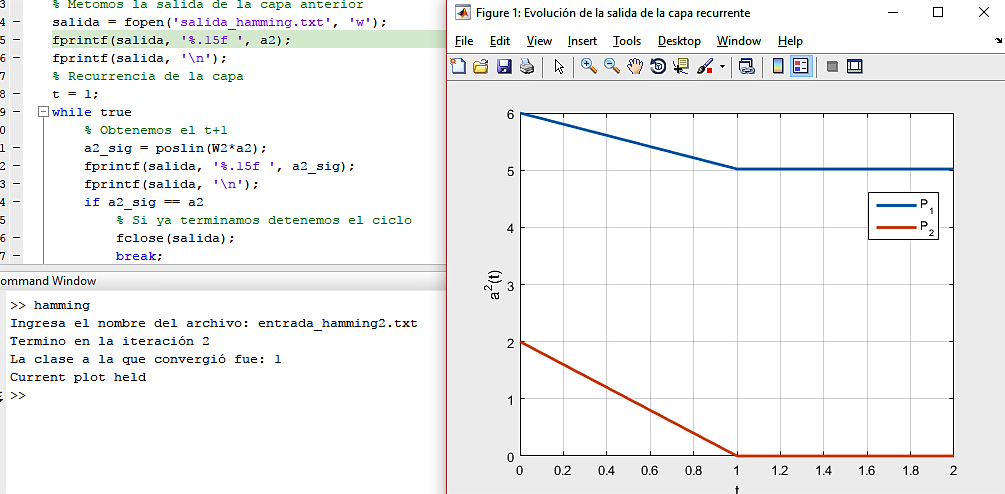
\includegraphics[width=16cm]{img/hamming/hamming2.png}
            \caption{Prueba 2 de la red Hamming.}
            \label{fig:hamming2}
        \end{center}
    \end{figure}
    Después del procesamiento de estos datos se pudo clasificar correctamente el vector de entrada, a la red le tomo dos iteraciones logar converger y a la clase a la que convergió fue la 1, esto se puede observar a detalle en la evolución de las salidas de la capa recurrente que se encuentra en la figura \ref{fig:hamming2}.
    \newline
    \textbf{Experimento 3.} En este ultimo experimento se utilizo un archivo llamado \emph{entrada\_hamming3.txt} para poder ingresar los datos a la red. El conjunto de vectores prototipo fue el siguiente.
    \[ \left\lbrace \boldsymbol{p_1} = \left[\begin{array}{c}-1\\ 1\\ 1 \\ 1 \\ 1 \end{array}\right], \boldsymbol{p_2} = \left[\begin{array}{c}-1\\ -1\\ 1 \\ -1 \\ 1 \end{array}\right], \boldsymbol{p_3} = \left[\begin{array}{c}1\\ 1\\ -1 \\ -1 \\ -1 \end{array}\right], \boldsymbol{p_4} = \left[\begin{array}{c}-1\\ -1\\ -1 \\ -1 \\ -1 \end{array}\right], \boldsymbol{p_5} = \left[\begin{array}{c}1\\ 1\\ 1 \\ 1 \\ 1 \end{array}\right] \right\rbrace \]
    El vector de prueba que se utilizo fue.
    \[ \boldsymbol{p} = \left[\begin{array}{c}1\\ -1\\ 1 \\ -1 \\ 1\end{array}\right] \]
    El utilizar estos valores produjo que la arquitectura de la figura \ref{fig:hamming-diagrama2} tuviera los siguientes valores.
    \begin{align*}
    R = 5 \implies \boldsymbol{b} = \left[\begin{array}{c}5 \\5 \\ 5 \\ 5 \\ 5\end{array}\right] && S = 5 && \boldsymbol{W} = \left[\begin{array}{c}\boldsymbol{p^{T}_1}\\ \boldsymbol{p^{T}_2} \\ \boldsymbol{p^{T}_3} \\ \boldsymbol{p^{T}_4} \\ \boldsymbol{p^{T}_5}\end{array}\right]
    \end{align*}
    \begin{figure}[H]
        \begin{center}
            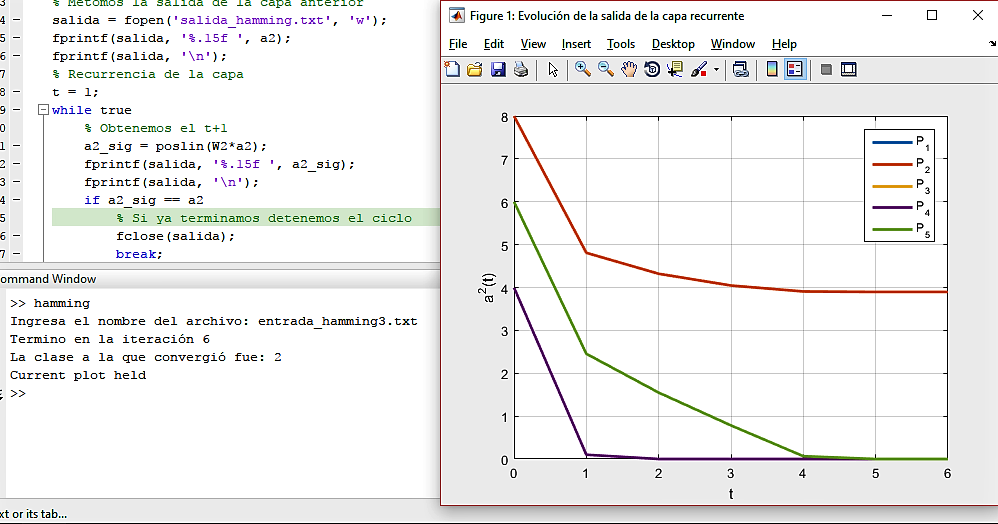
\includegraphics[width=16cm]{img/hamming/hamming3.png}
            \caption{Prueba 3 de la red Hamming.}
            \label{fig:hamming3}
        \end{center}
    \end{figure}
    Como se puede observar en la figura \ref{fig:hamming3} la red pudo converger a un resultado satisfactorio en la iteración 6 dando como resultado que el vector de prueba perteneciera a la clase 2 debido a que es la única salida que tiene un valor diferente a 0.
    \newpage
    \section{Discusión de resultados}
    Es fácil darse cuenta que los resultados fueron correctos debido a la simplicidad de esta red, estos pueden ser comprobados fácilmente por uno mismo las únicas posibles diferencias que pueden existir son al elegir los valores que son aleatorios como lo son en este caso épsilon. Esta variable de la red podría producir que la red termine de trabajar en un mayor o menor numero de iteraciones.
    
    Otro punto importante a mencionar es el como el funcionamiento de la red es muy evidente en las gráficas de la evolución de sus salidas (véanse figuras \ref{fig:hamming1}, \ref{fig:hamming2}, \ref{fig:hamming3}). Donde como era de esperarse la neurona con el valor inicial más alto es la que disminuye más lento mientras que el resto lo hace con una pendiente más pronunciada. Esto se debe a que el vector de entrada tiene más valores en común con algunos vectores que con otros (menor distancia de Hamming), de nuevo esto se ve reflejado en la gráfica donde a mayor numero de puntos en común mayor valor inicial en la capa recurrente.
    
    Por ultimo, aquellos vectores con misma distancia de Hamming con respecto al vector de entrada tienen el mismo comportamiento en la gráfica.
    \newpage
    \section{Conclusiones}
    La primera ventaja que surge al usar una red Hamming es la facilidad que la rodea desde la teoría y su funcionamiento, el cual a lo largo de esta practica ha sido evidente que es bastante sencillo de entender y aplicar, hasta su implementación la cual es incluso intuitiva.
    \\\\
    Esta facilidad es lo que hace que sea una muy buena opción para problemas pequeños donde las variables se puedan restringir a solamente dos posibles valores.
    \\\\
    Sin embargo su propia simplicidad restringe mucho los posibles casos en los que podemos aplicarla o en el mejor de los casos hace que tengamos que procesar y darle cierta estructura a los datos que estamos manejando, esto debido a que solo puede trabajar con problemas de tipo binario lo cual en casos donde tenemos una variable que puede tomar más valores tendríamos que hacer una división de esa variable en más variables para poder reducir los valores que esta pude tomar, cosa que puede resultar en una tarea imposible, o en su defecto operar nuestros datos por grupos lo que haría nuestra clasificación una tarea más complicada de lo que debería.
    \\\\
    A pesar de esta gran desventaja el estudio de esta red neuronal es de gran importancia ya que al ser de las redes competitivas más sencillas es una buena introducción al estudio de este tipo de redes.
    \newpage
    \bibliographystyle{apalike}
    \bibliography{bibliografia}
    \newpage
    \section{Anexo}
\begin{lstlisting}
% Cada elemento del vector de entrada tiene solo dos posibles valores
opcion = input('Ingresa el nombre del archivo: ', 's');
archivo = dlmread(opcion);
tam = size(archivo);
% Tam de nuestros vectores prototipo
R = tam(2);

% Numero de neuronas, corresponde a cada vector prototipo
S = tam(1) - 1;

% Vector a clasificar
p = archivo(S+1, :)';

% Las filas de W1 son los vectores prototipos
% Inicializacion de W1
W1 = archivo(1:S, :);

% Cada elemento del bias es el tam del vector prototipo
% Inicializacion del bias
b1 = ones(S, 1) * R;

% Propagamos hacia adelante
a1 = purelin((W1*p)+b1);
% Fin de la capa feedforward

%Inicio de la capa recurrente
a2 = a1;
% Obtencion del valor epsilon 0 < epsilon < 1/(S-1)
epsilon = round(rand(1)*1/(S-1), 4); 
% Inicializacion y llenado de la W2 de la capa recurrente
W2 = ones(S, S);
for i = 1:S
    for j = 1:S
        if i==j
            W2(i, j) = 1;
        else
            W2(i, j) = -epsilon; 
        end;
    end;
end;

% Aqui se guardara la salida de la capa recurrente
% Metomos la salida de la capa anterior
salida = fopen('salida_hamming.txt', 'w');
fprintf(salida, '%.15f ', a2);
fprintf(salida, '\n');
% Recurrencia de la capa
t = 1;
while true
    % Obtenemos el t+1
    a2_sig = poslin(W2*a2);
    fprintf(salida, '%.15f ', a2_sig);
    fprintf(salida, '\n');
    if a2_sig == a2
        % Si ya terminamos detenemos el ciclo
        fclose(salida);
        break;
    else
        % Siguiente iteracion
        a2 = a2_sig;
    end;
    t = t + 1;
end;

% Fin de la capa recurrente
fprintf('Termino en la iteracion %d\n', t);
v = 1;
for ite = a2'
    if ite ~= 0
        break;
    else
        v = v+1;
    end;
end
fprintf('La clase a la que convergio fue: %d\n', v);
% Imprimir datos y graficar la salida de a2
a2_recurrente = dlmread('salida_hamming.txt');
figure('Name', 'Evolucion de la salida de la capa recurrente');
plot(0:t, a2_recurrente, 'LineWidth', 2);
hold;
grid;
xlabel('t');
ylabel('a^2(t)');
etiquetas = cell(1, S);
for i = 1:S
    etiquetas{i} = ['P_' num2str(i)];
end;
legend(etiquetas);
\end{lstlisting}
\end{document}